\documentclass{beamer}

\usepackage[utf8]{inputenc}
\usepackage[russian]{babel}  % Russian layout
\usepackage{amsmath,mathrsfs,amsfonts,amssymb}
\usepackage{graphicx, epsfig}
\usepackage{subfig}
\usepackage{floatflt}
\usepackage{comment}
\usepackage{epic,ecltree}
\usepackage{mathtext}
\usepackage{fancybox}
\usepackage{fancyhdr}
\usepackage{enumerate}
\usepackage{epstopdf}
\usepackage{xcolor}
\usepackage[]{algorithm2e}
\usepackage{Iv_commands_slides}

\DeclareMathOperator{\argmin}{arg\!min}
\DeclareMathOperator{\argmax}{arg\!max}

\usetheme{Boadilla}%{Singapore}%{Warsaw}%{Warsaw}%{Darmstadt}%{Frankfurt}%{Dresden}
%\definecolor{beamer@blendedblue}{RGB}{15,120,80}
%\definecolor{light-gray}{rgb}{0.8,0.8,0.8}
\usecolortheme{wolverine}
%\setbeamercolor{frametitle}{fg=Brown,bg=brown!20}
%\setbeamercolor{section in head/foot}{bg=brown}
%\setbeamercolor{author in head/foot}{bg=brown}
%\setbeamercolor{date in head/foot}{fg=brown}

\usecolortheme{sidebartab}
\useinnertheme{circles}
%----------------------------------------------------------------------------------------------------------
\title[\hbox to 56mm{\hfill\insertframenumber\,/\,\inserttotalframenumber}]
{Мультимоделирование SVM}
%\author[С. Иванычев, А. Адуенко]{\large \\Сергей Иванычев, Александр Адуенко}
\author[С. Иванычев \& А. Адуенко]
       {\parbox[t]{1.5in}{Сергей Иванычев \\{\scriptsize   \texttt{sergeyivanychev@gmail.com}}} \and 
        \parbox[t]{1.5in}{Александр Адуенко \\  \and {\scriptsize   \texttt{aduenko1@gmail.com}}}}
\institute[МФТИ]{Московский физико-технический институт \\
    Факультет управления и прикладной математики\\
    Кафедра <<Интеллектуальные системы>>
}
\date{\footnotesize{}}
%----------------------------------------------------------------------------------------------------------
\begin{document}
%----------------------------------------------------------------------------------------------------------

\begin{frame}
%\thispagestyle{empty}
\titlepage
\end{frame}
%-----------------------------------------------------------------------------------------------------

\section{Предпосылки}
\begin{frame}{Предпосылки. Комбинирование алгоритмов.}
	\begin{block}{Понятие}
        \textbf{Сильный классификатор} --- $\mathrm{|AUC - 0.5| \gg 0}$ во многих реальных задачах.
    \end{block}
    Примеры: SVM, логистическая регрессия, Lasso...
    \begin{block}{Понятие}
        \textbf{Слабый классификатор} --- $\mathrm{|AUC - 0.5| > 0}$ в большинстве задач
    \end{block}
    Примеры: решающий пень...
		
\end{frame}
\begin{frame}{Предпосылки. Комбинирование алгоритмов.}
	\begin{block}{Комбинирование сильных классификаторов}
		\begin{itemize}
			\item Простое голосование
			\item Линейная комбинация
			\item ...
		\end{itemize}
    \end{block}
    
    \begin{block}{Комбинирование слабых классификаторов}
		\begin{itemize}
			\item Bagging
			\item Boosting
		\end{itemize}
    \end{block}	
\end{frame}

\begin{frame}{Предпосылки. Задача}

     \begin{block}{Вопросы}
        Может ли нелинейная комбинация классификаторов решать задачу лучше, чем каждый классификатор по отдельности?
     \end{block}
     
     Сужение задачи: модели --- SVM с разными ядрами, комбинирующий алгоритм --- логистическая регрессия. 
\end{frame}
\begin{frame}{Цели исследования}
    \begin{block}{Цели}
        \begin{itemize}
        	\item Построить лучшую по сравнению с отдельными моделями комбинацию (супермодель)
        	\item Установить связь между множествами опорных объектов и схожестью классификаторов
        	\item Использовать знание множеств опорных объектов для улучшения комбинации
        \end{itemize}
    \end{block}
\end{frame}
\section{Простановка задачи}
\begin{frame}{Постановка задачи}
Пусть $X^l = (x_i, y_i)_{i=1}^l, x \in R^n, y \in \{\pm 1\}$.
     \begin{block}{Определения}
        \textbf{$S$-я модель} --- SVM с ядром $K_s$ из множества ядер:
    	$$
    	\mathcal{K} = \{K_j\}_{j=1}^m
    	$$
    	
    	\textbf{Отступ} --- значение дискриминантной функции на объекте
    	$$
    	M_s = \sum_{i=1}^l \lambda_i y_i K_s(x_i, x) - w_0
    	$$
     \end{block}
\end{frame}
\begin{frame}{Постановка задачи}
	$$
	M = \begin{pmatrix}
		M_1 & \ldots & M_s
	\end{pmatrix}
	$$
	--- матрица отступов, новая матрица <<объект-признак>>.
	
	Пусть $\mathcal{A}$ -- множество алгоритмов классификации.
	$$
	\mathcal{A} = \{a(x) = g(x, \theta) | \theta \in \Theta\}
	\;\; g: R^m \to Y
	$$
	\begin{block}{}
		Пару $(g, \mathcal{K})$ будем называть \textbf{супермоделью}.
	\end{block}
	\begin{block}{Задача выбора алгоритма комбинирования}
		$$
		L(y, g(M(X^l), \theta)) \to \min_{\Theta} 
		$$
	\end{block}
	Где $L$ --- функционал качества (в нашем случае AUC)
\end{frame}
%----------------------------------------------------------------------------------------------------------
\begin{frame}{Литература}
    \begin{enumerate}
        \footnotesize {
        \item
            Corinna Cortes and Vladimir Vapnik. Support-Vector Networks. 1995
        \item
        Alex J Smola et al. A Tutorial on Support Vector Regression. 2004
        \item
        Rauf Izmailov, Vladimir Vapnik and Akshay Vashist. Multidimensional Splines with Infinite Number of Knots as SVM Kernels. 2013
            }
        \item
        D. Gorgevik и D. Cakmakov. Handwritten Digit Recognition by Combining SVM Classiers. 2005
        \item 
        Salah Althloothi и др. Human activity recognition using multi-features and multiple kernel learning. 2014
        \item
        S.S. Bucak, R. Jin и Ak. Jain. Multiple Kernel Learning for Visual Object Recognition: A Review. 2014
     \end{enumerate}
\end{frame}
% ==============================================================================
\section{Модельные расстояния}
\begin{frame}{Связь между разными расстояниями.}

Необходимо найти способ определять схожие модели, то есть дающие схожие результаты, 
 чтобы не включать таковые в супермодель. 

\begin{block}{Расстояния}
	\textbf{Опорным расстоянием} $\rho_S(K_i, K_j)$ на выборке $X^l$ будем называть функцию:
$$
\rho_M(K_i, K_j, X^l) = \frac{\#\sbrs{\mathrm{SV}_i \;\Delta\; \mathrm{SV}_j}}
{\#\sbrs{\mathrm{SV}_i \cup \mathrm{SV}_j}}
$$
%$\mathrm{SV}_j$ --- множество опорных объектов на $j$-м ядре, $\Delta$ --- симметрическая разность.

	\textbf{Отступным расстоянием} $\rho_M(K_i, K_j)$ будем называть следующую функцию
$$
\rho_M(K_i, K_j, X^l) = 1 - \mathrm{corr}(M_i, M_j)
$$	
%где под $M_i$ понимается вектор отступов соответственного SVM, а функция $\mathrm{corr}(\cdot, \cdot)$ --- корреляция Пирсона. 
\end{block}

Связаны ли эти расстояния? Проанализируем эволюцию распределения пар расстояний в зависимости от параметра регуляризации.

\end{frame}
% ==============================================================================
\begin{frame}{Эксперимент. Ядра и данные.}

В качестве исходных данных взяты датасеты German Credits, Wine и Heart disease из UCI.

Ядра:

\begin{itemize}
    \item Линейное
    \item Полиномиальное (степени 3, 4, 5)
    \item RBF-ядро ($\gamma \in \{0.0001, 0.001, 0.01, 0.1, 1\}$)
    \item {INK-spline ядро}
\end{itemize}

    
\end{frame}
% ==============================================================================
\begin{frame}{Эксперимент. German credit}

\begin{figure}[H]
      \center{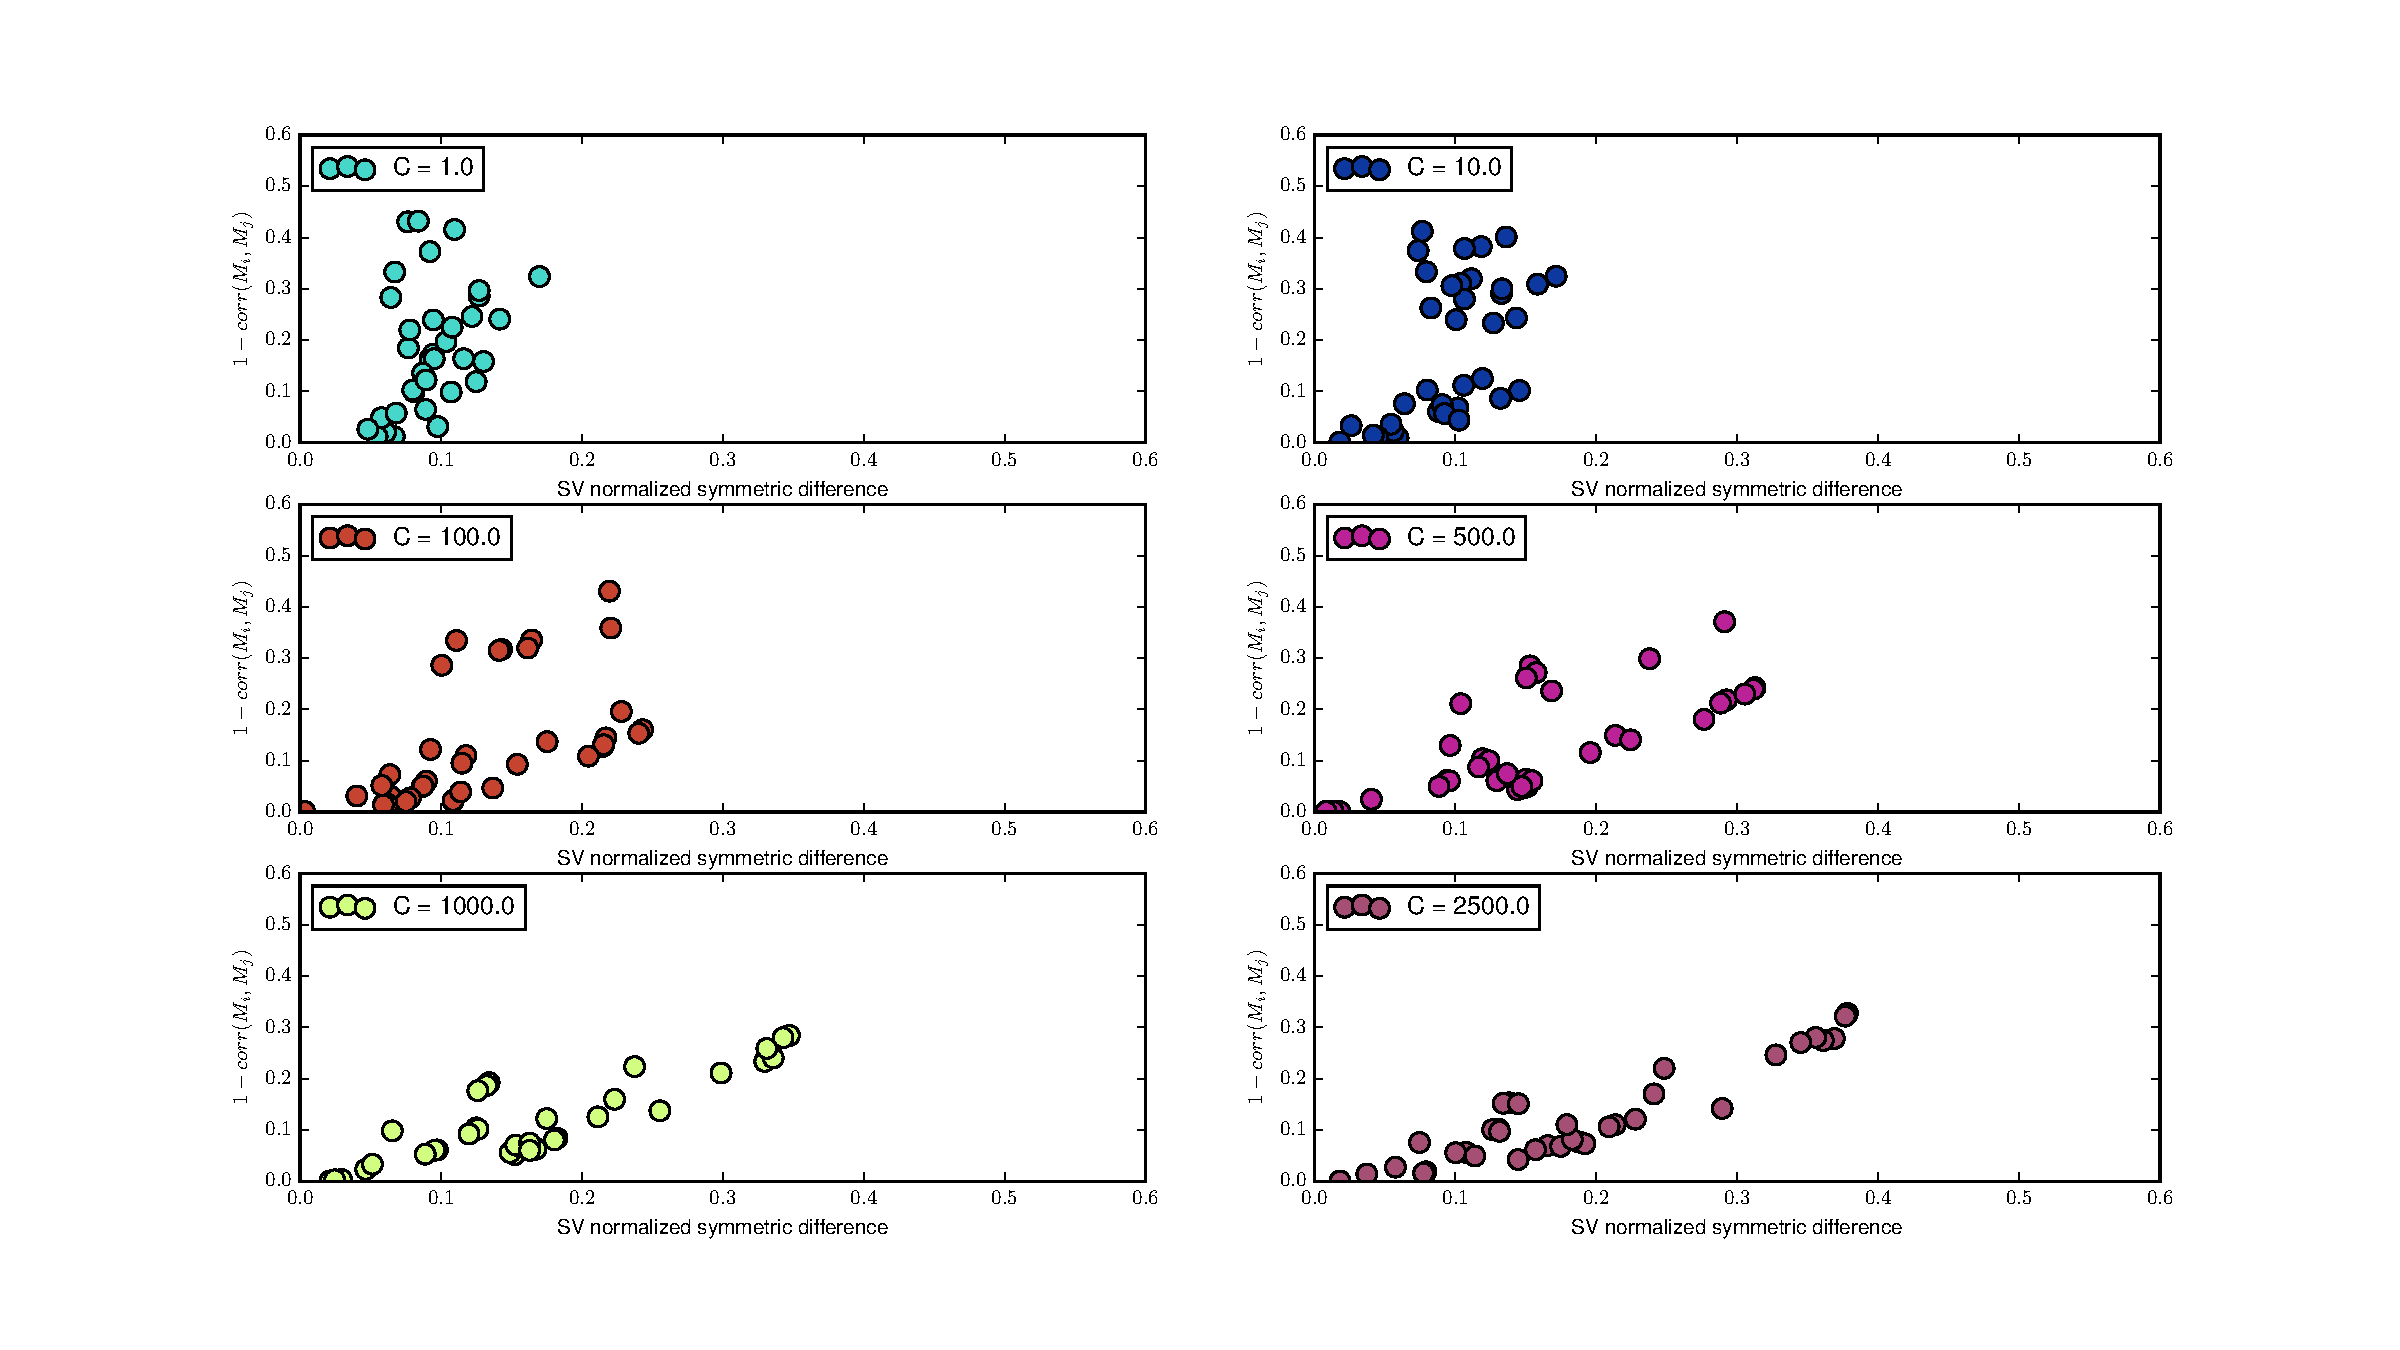
\includegraphics[width=\textwidth]{german.pdf}}
      \caption{German credit}
\end{figure}

\end{frame}

\begin{frame}{Эксперимент. German credit}

\input{german.tex_table}
\end{frame}

\begin{frame}{Эксперимент. Wine}

\begin{figure}[H]
      \center{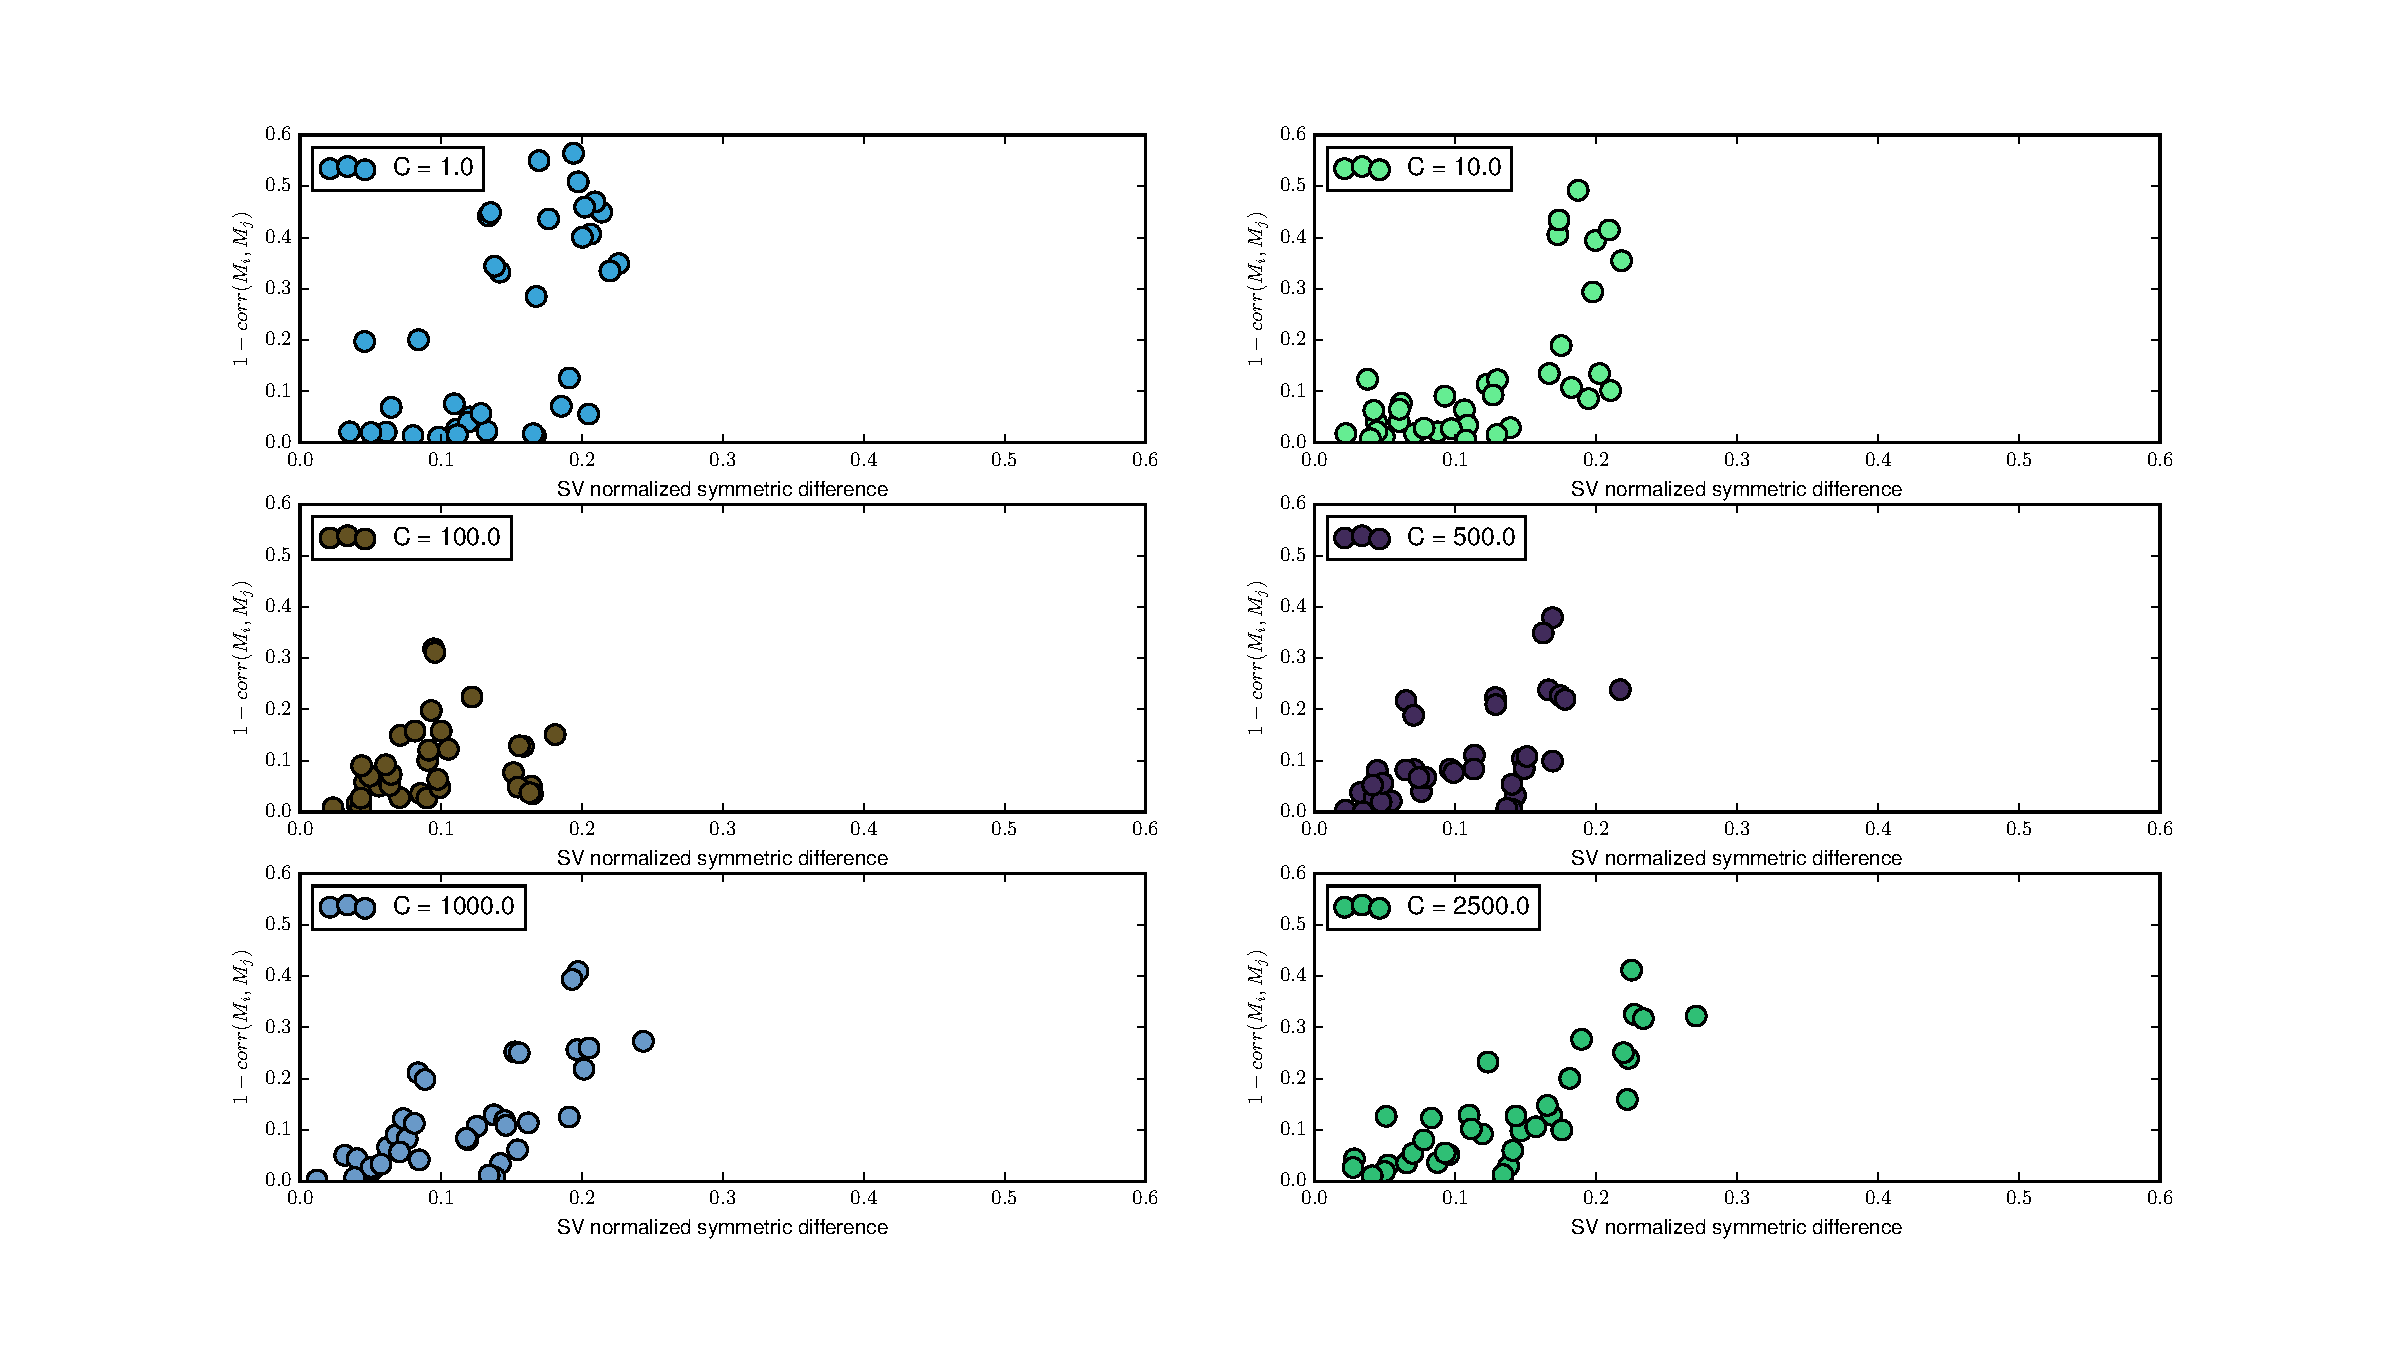
\includegraphics[width=\textwidth]{wine.pdf}}
      \caption{Wine}
\end{figure}

\end{frame}
\begin{frame}{Эксперимент. Wine}
\input{wine.tex_table}
\end{frame}
\begin{frame}{Эксперимент. Heart disease}

\begin{figure}[H]
      \center{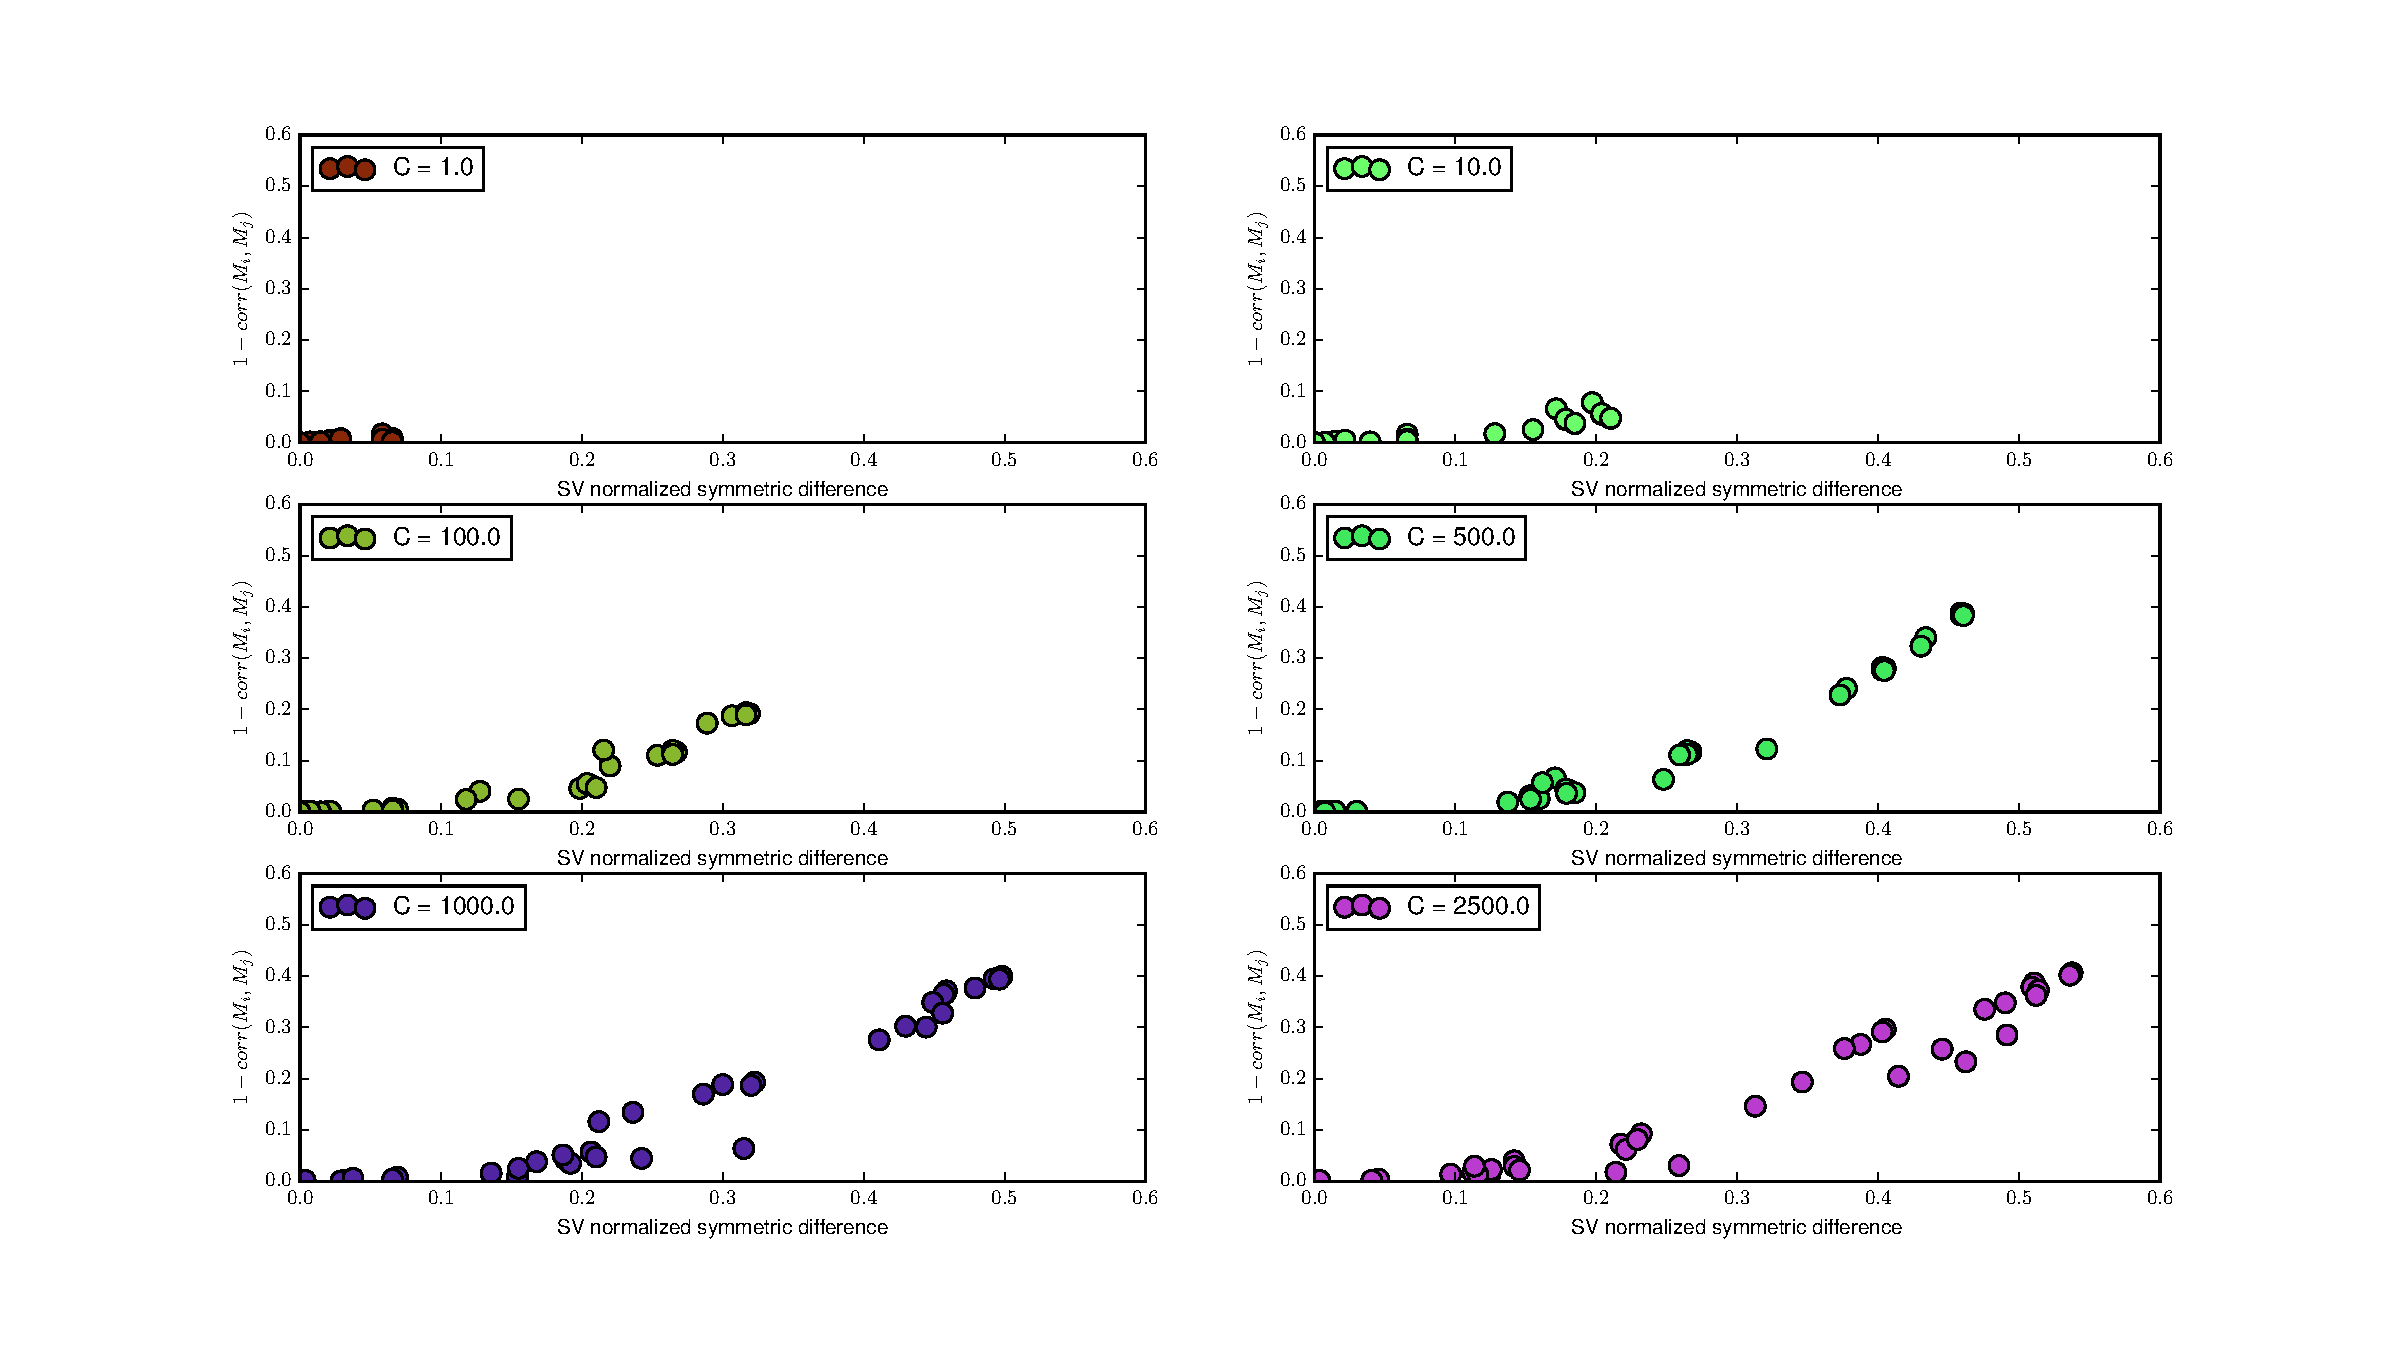
\includegraphics[width=\textwidth]{heart.pdf}}
      \caption{Heart disease}
\end{figure}

\end{frame}

\begin{frame}{Эксперимент. Heart disease}

\input{heart.tex_table}

\end{frame}
\begin{frame}{Результаты эксперимента}
\begin{itemize}
  \item С ростом константы регуляризации расстояние между ядрами и расстояние между
  их отступами лучше коррелируют между собой.
  \item При высоких параметре регуляризации коэффициент корреляции Пирсона 
  достигает более $0.8$, то есть расстояния практически линейно зависят друг от друга.
%  \item Вектора средних ядерных и отступных расстояний кореллируют по-разному на различных датасетах (на Wine и Heart корелляции Пирсона $0.85$ и $0.99$ соответственно, на German --- $-0.92$).
\end{itemize} 

    \begin{block}{Вывод}
Если множества опорных объектов пары классификаторов похожи
    , то и векторы отступов похожи
    \end{block}
\end{frame}
\newcommand{\Xtrain}{X_\text{train}}
\newcommand{\Xval}{X_\text{val}}
\newcommand{\Xtest}{X_\text{test}}
\newcommand{\ytrain}{y_\text{train}}
\newcommand{\yval}{y_\text{val}}
\newcommand{\ytest}{y_\text{test}}
\newcommand{\SVM}{\mathrm{SVM}}
\newcommand{\Logregr}{\mathrm{Logregr}}
\newcommand{\predictprobability}{\mathrm{predict\_probability}}
\newcommand{\fit}{\mathrm{fit}}
\newcommand{\margin}{\mathrm{margin}}
\section{Супермоделирование}
\begin{frame}{Построение супермодели}
	Обозначения: $\Xtrain, \Xtest, \ytrain, \ytest$
	\begin{block}{}
	\begin{algorithm}[H]
%	\LinesNumbered
	\tcc{Обучение
	}
	$\SVM.\fit(\Xtrain, \ytrain)$\;
	$M_{\text{train}} \leftarrow \SVM.\margin(\Xtrain)$\;
	$\Logregr.\fit(M_\text{train}, \ytrain)$\;
	\tcc{Прогнозирование
	}	
	$M \leftarrow \SVM.\margin(\Xtest)$\;
	$\Logregr.\predictprobability(M)$\;
	\caption{Наивная логистическая регрессия}
	\end{algorithm}
	\end{block}
	
	Плохо! Если во множестве моделей есть переобученный классификатор, то супермодель будет также переобучена
\end{frame}
\begin{frame}{Построение супермодели}
	\begin{block}{}
	\begin{algorithm}[H]
%	\LinesNumbered
	\tcc{Обучение
	}
	$\Xtrain, \Xval \leftarrow \mathrm{split}(X)$\;
	$\SVM.\fit(\Xtrain, \ytrain)$\;
	$M_{\text{val}} \leftarrow \SVM.\margin(\Xval)$\;
	$\Logregr.\fit(M_\text{val}, \yval)$\;
	\tcc{Прогнозирование
	}	
	$M \leftarrow \SVM.\margin(\Xtest)$\;
	$\Logregr.\predictprobability(M)$\;
	\caption{Стэкинг}
	\end{algorithm}
	\end{block}
	
	Уже лучше, однако не понятно, как интерпретировать отрицательные веса в логистической регрессии.
\end{frame}
\begin{frame}{Построение супермодели}
	Используем \textbf{робастную логистическую регрессию}. Преобразуем задачу оптимизации:
	
	$$
		R(w) + C \sum_{i=1}^n \log(\exp(- y_i (X_i^T w + c)) + 1) \to \min_{w \geq 0, c}
	$$
	
	Получаем вектор неотрицательных весов
\end{frame}
\begin{frame}{Выводы}
	Эксперимент был проведен на датасетах Housing, Heart, German и синтетически сгенерированном. С учетом примененных эвристик, таких как:
	\begin{itemize}
	\item 	Использование классификаторов только из интервала $[\mathrm{AUC_\text{best}}, \mathrm{AUC_\text{best}} - \delta]$
	\item Повторное обучение $\SVM$ на $X$, после обучения регрессии
	\item Использование $l_1$-регуляризации для логистической регрессии
	\end{itemize}
	пока не удалось получить супермодель с устойчивым выигрышем. 
	
	$$
	\mathrm{AUC}_{\text{best}} - 
	\mathrm{AUC}_{\text{super}} \approx 0.002
	$$
	\begin{block}{Направления дальнейшей работы}
		\begin{itemize}
			\item Усовершенствование или исправление комбинирующего алгоритма.
			\item Использование расстояний между моделями для улучшения качества предсказаний.
		\end{itemize}
	\end{block}

\end{frame}
\begin{frame}{Code sharing}

		Исходный код проекта написан на языке Python 3.5. Код и данные доступны по ссылке:
		{\tiny
		\href{https://sourceforge.net/p/mlalgorithms/code/HEAD/tree/Group374/Ivanychev2016SVM_Multimodelling/}{https://sourceforge.net/p/mlalgorithms/code/HEAD/tree/Group374/Ivanychev2016SVM\_Multimodelling/}	}
	
	Супермодель представлена в виде объекта \texttt{SVMSupermodel} и обладает стандартным интерфейсом классификаторов библиотеки \texttt{scikit-learn}. 
	
	Основная статья, а также подробная документация доступна в папке с проектом.
\end{frame}



\end{document} 
